\section{Multichannel RPL Protocol}
\label{sec:multichannel}
Multichannel RPL concentrates on finding the best channels for nodes to listen and transmit on, given policies that needs to be complied. 

\subsection{Overview}

%\explain the ideas (state machine?), reasons for doing

The design of Multichannel RPL are based on several crucial observations:

\begin{itemize}
\item Channel assignment - Sensors have limited memory and battery capabilities. In order to maximise the sensors lifetime, a centralised LPBR that has larger memory and fully powered is opted. LPBR has a complete knowledge of the topology which enables it to make good channel assignment decisions based on the criteria that are explained in the next part. 
%LPBR assigns channel to the nodes.
%This centralised processes at the LPBR enable the other nodes that are battery powered to minimise the use of the energy in packets transmission. LPBR is fully powered which is the main reason for placing intelligence on it.
%LPBR keeps track of the channel conditions based on the feedback it receives from the nodes. All intelligence is done at LPBR.
%by considering load balancing in channels.

\item Interference - External interference cannot be predicted, thus channels cannot be allocated beforehand as it varies over time and locations. It is impossible to determine a single channel that is free from interference at any location. Our protocol checks the channel condition each time before deciding on a channel change to reduce interference and maximise throughput.

\item Frequency diversity - RPL is typically used with ContikiMAC which is a single channel protocol. By using multichannel, we increase the robustness of the network towards interference. However, applying multichannel to the existing RPL may hinder neighbour detection and RPL processes to maintain the network topology as it does not switch to the correct channel. We overcome this problem by enabling unicast in neighbour detection and RPL control messages. We assume that no new nodes should join the topology after the initial setup.
%we need to ensure the node knows the correct channel to reach the neighbours. RPL forms and maintains the network topology through its control messages. Applying multichannel to the existing RPL may hinder neighbour detection and RPL processes and it does not have any means of switching to the correct channel. 
\end{itemize}

Multichannel RPL focuses on the network and application layer of the protocol. This allows channel assignment decisions to be made thoroughly without being limited by the low layer complexity. The channel assignment processes take place once the topology tree has been formed by LPBR and stabilise.

%Figure 1 shows the design of Multichannel RPL. The states are explained in the next sections.

%\begin{figure}
%\centering
%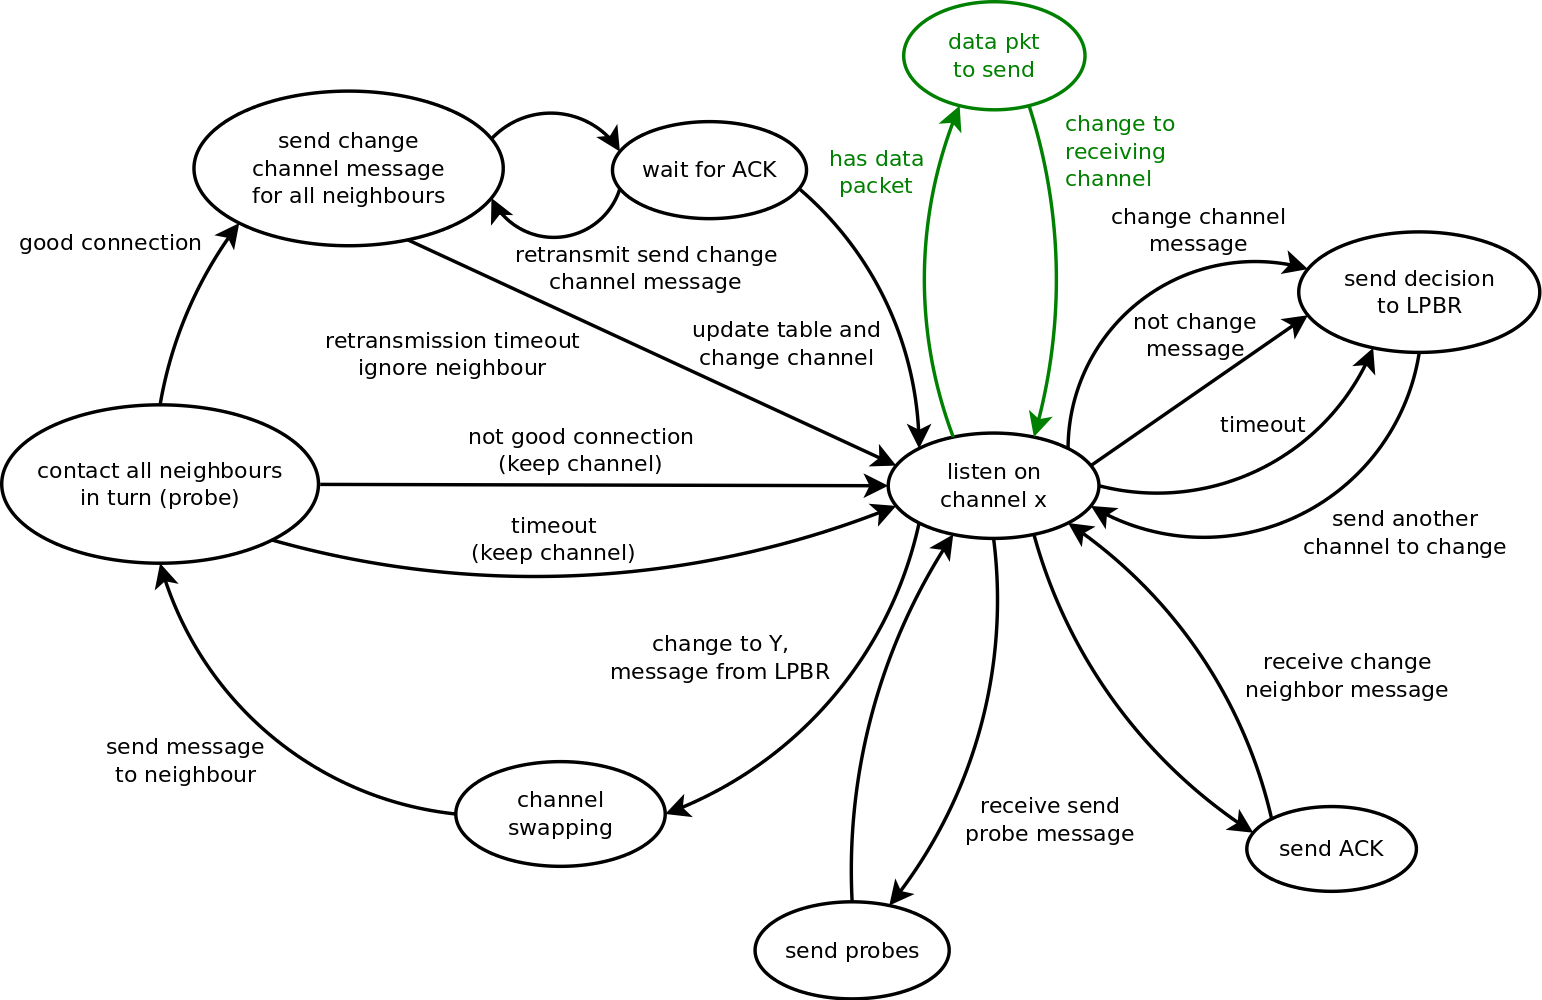
\includegraphics[height=7.2cm]{stateDiagram}
%\caption{State machine for channel switching.}
%\label{fig:example}
%\end{figure}

\subsection{Channel Selection Strategy}

%//LPBR decides the channel; random at first (or maybe not) and then based on probing that were done previously stating the condition of channels.
%//be more detail - better description of 2-hop strategy reasoning. %WHY?? keep them not to interference so much with each other
LPBR uses a two hops neighbour strategy to select a channel to be assigned to a node. This allows fair load balancing on the channels and reduces congestion on the channel that could occur when several nearby nodes start transmitting at similar time. A sensor node integrated an onboard antenna that covers a transmission range of 50 metres indoor and 125 metres outdoors between the sensors. Two hops from the node would cover some ranges between the nodes to reduce transmission interference to a minimum. This allows transmission to happen at the same time without the risk of packet loss due to collision. 

However, at initialisation, all nodes are initialised to channel 26 by default. The nodes need to be on the same channel for neighbour discovery and enable RPL to exchange control messages that are required to form an optimised topology before channel assignments can take place. The nodes will only be on the same channel once during the initial setup. Channel 26 is chosen as the initial channel as it usually does not overlap with WiFi and is relatively in a cleaner frequency than the other channels. The studies in \cite{chrysso}\cite{micmac}\cite{watteyne} use several channels in their experiments and have channel 26 in common.
	
%**TWO HOP COLOURING STRATEGY?
%\subsubsection{Two Hops Neighbour Strategy -}


%//how it works?
%During the initial setup, LPBR does not have any knowledge of the channels condition. All channels are assumed to be available to be used. LPBR assigns a random channel to a node. The node that receives the channel change message will inform all of its neighbour of its new channel. The neighbours will update their neighbour table to hold the new channel value as the node current channel for transmission. The neighbour nodes will in turn, send probing messages.

\iffalse
\begin{algorithm}
\caption{Two hops neighbour strategy}
\begin{algorithmic} 
\STATE $newChannel \neq currentChannel$
\STATE $newChannel \leftarrow x$

\REQUIRE\emph{first hop}{}:
\WHILE {$retry \neq 4$}
\IF{$node = LPBRneighbour$}

\IF {$newChannel \neq LPBRChannel$}
\STATE {\emph {second hop}}
\ELSE
\STATE $newChannel \leftarrow y$
\ENDIF

\ELSE [$node = neighbourNeighbour$]
\IF {$newChannel \neq neighbourChannel$}
\STATE {\emph {second hop}}
\ELSE
\STATE $newChannel \leftarrow y$
\ENDIF
\ENDIF
\ENDWHILE


\REQUIRE\emph{second hop}{}:
\WHILE {$retry \neq 4$}
\IF{$node = LPBRneighbour$}

\IF {$newChannel \neq LPBRneighboursChannel$}
\STATE $newChannel \leftarrow OK$
\ELSE
\STATE $newChannel \leftarrow y$
\ENDIF

\ELSE [$node = neighbourNeighbour$]
\IF {$newChannel \neq neighbourNeighboursChannel$}
\STATE $newChannel \leftarrow OK$
\ELSE
\STATE $newChannel \leftarrow y$
\ENDIF
\ENDIF
\ENDWHILE
\end{algorithmic}
\end{algorithm}
\fi

In two hops neighbour strategy, LPBR chooses a random channel from channel 11 to 26 for a node unless LPBR has full knowledge of the channels condition. If LPBR has knowledge of all the channels, LPBR can limit the channels range to consider only channels that the node has used in the past that gives good transmission results. LPBR keeps the information of each node neighbours and channels in a table. Before LPBR sends a channel change message to the node, it first checks if the node is LPBR neighbours. If it is, LPBR checks if the new channel value is the same as LPBR channel. If it is not, LPBR checks if the node is a neighbour of other nodes. The new channel is compared with the current channel. If the channels are the same, the first hop of the two hop strategy has failed. LPBR will try going through the same steps with another new channel.

If the first hop succeeds, LPBR will check the nodes that are two hops away from the node the new channel is for. If the node is LPBR neighbour, LPBR checks the new channel value with all LPBR neighbours channels. Otherwise, the node neighbours neighbours channels are checked. If the channel values are not the same, LPBR will send the new channel value to the node to proceed with channel quality checking. If the two hops failed, LPBR retries with a new channel value. The steps from the first hop is repeated. LPBR tries to find the channel that is two hops free within four tries. If a two hops free channel is not found, the default channel 26 is used.

\subsection{Channel Quality Checking}
%channel quality check = probing
%//Channel condition is checked by probing before deciding to switch unless LPBR has the information regarding the specific channel based on probing that were done previously.

The channel quality checking is invoke each time the node receives the channel change message from LPBR. The node informs all the route neighbours in turn, of the new channel it will be listening on. The route neighbours will update their neighbour table to hold the new channel value as the node current channel for transmission. The node sends a message to the route neighbour to send probes and switches to the listening channel ready to receive any incoming messages. The node's route neighbour starts sending the probe messages to the node and the node collects the information on the success or failure rate of the channel. These information is then, sent to LPBR to updates LPBR's knowledge on the channel condition for the specific node and its neighbours. The node uses the results from probing to decide if the new channel is better than the current channel. All the neighbours and LPBR are informed of the decision and update the node's channel.

A channel is not chosen as a good channel to change into either if it timed out or the probing messages received are below a threshold. The node will revert to the previous channel as it is better than the new channel selected. The interference channel might be used by some nodes if during the probing, all probing messages are received. The channel change will be invoked again in this case.

Probing is an important part in making the channel changes decision. It gives a quick overview of the channel condition based on the number of probing messages received. It is worth noting that probing is only done between the node and the route neighbours. Neighbours that are not route neighbours will not use the node as a route during their transmission thus there is no need for probing to take place for those neighbours. However, the neighbours still need to know the channel value as RPL control messages are sent to neighbours directly without using the routes.
%***probing tries to avoid the interference channel.


%We could increase the number of probing messages by increasing the buffer size or the radio duty cycle (to be confirmed!!) but we chosen not to because increasing buffer size means that we will be using more memory which is not practical as we have limited memory available. If we increase the radio duty cycle, that would cost us more energy as the node will be awake more frequent and the nodes will not be in sync as they would have different radio duty cycle. That would increase the chance of packet loss. Our other option is to run the probing for a longer time.

%////FUTURE WORK?
%Even though external interference varies over time, it is unlikely that the channel quality fluctuates frequently within minutes that would affect the receiving success rate. Thus, the channel quality check is invoke on three (cases? situations?); on initialisation, when receiving LPBR channel change message and when the packet delivery ratio (PDR) drops. ***NOT SURE  


%****
%Each node keeps the counter of packets it has sent and received. It will send the information to LPBR periodically in order for LPBR to get a full view on the condition of the channels. LPBR will then decide if the node needs to change to another channel depending on the sent and received information. If the node does not perform well based on the number of received packets less than the number of packets being sent, LPBR will decide on a new channel the node needs to change into. The node will go through the channel changing processes to decide if the new channel is performing better than the previous channel before (settling?) for the new channel.

\subsection{Channel Switching}

%//explain LPBR that decides whether the nodes should stay on the same channel or switch to a new channel based on the information it gathers through nodes probing.

%State machine explanation should be here?

\begin{figure}
\centering
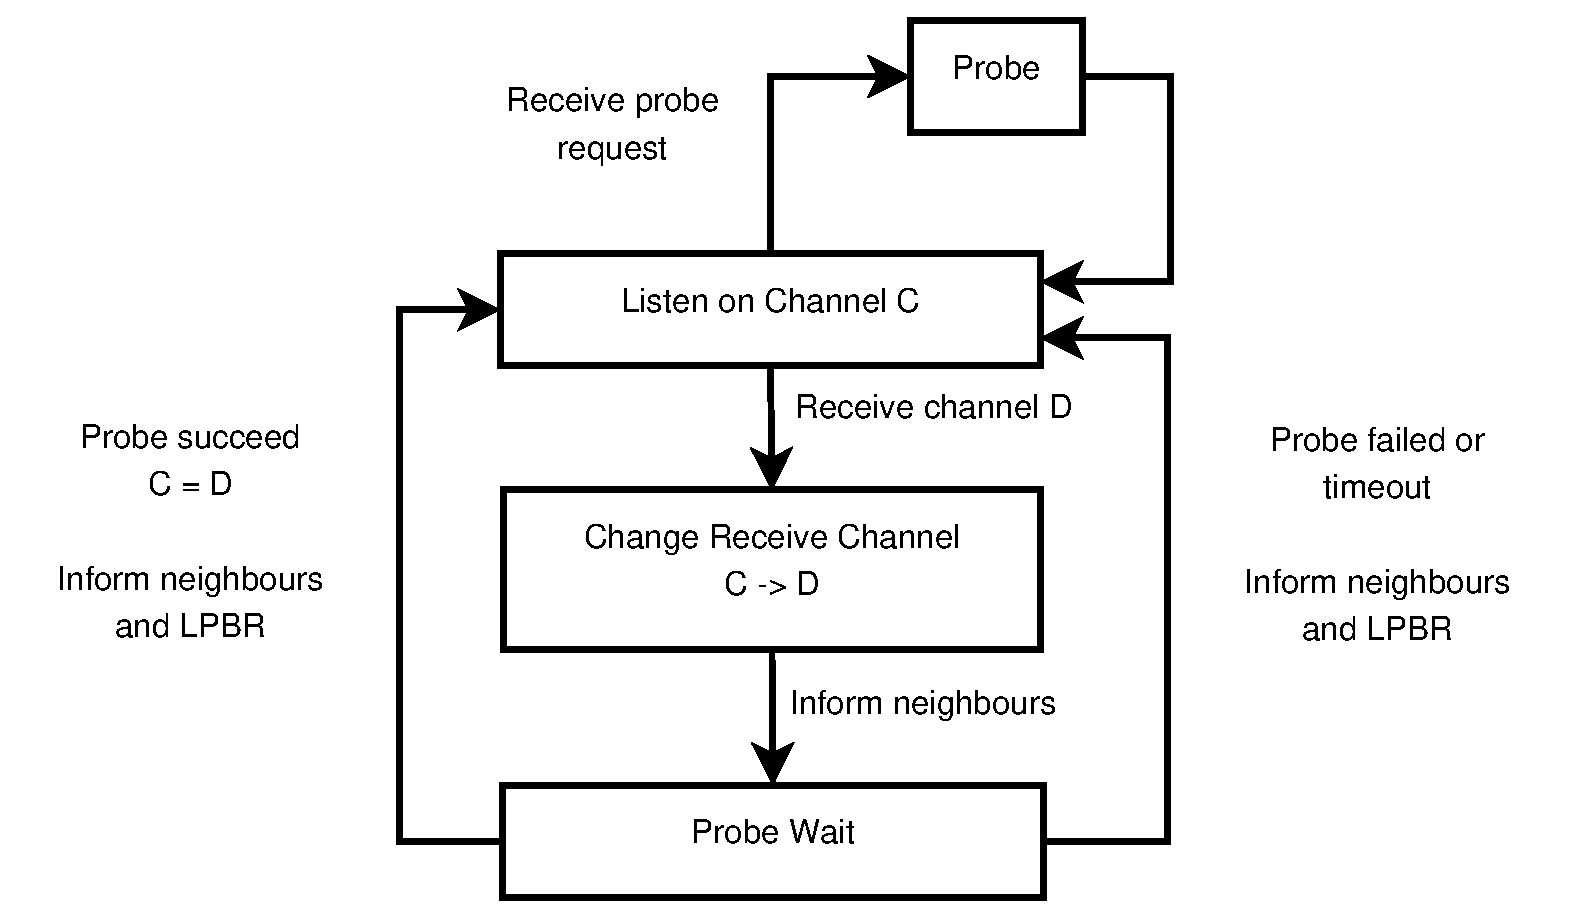
\includegraphics[width=3.5in]{Diagram1.eps}
\caption{Channel switching process}
\label{fig_sim}
\end{figure}

Figure 1 shows the states in channel switching. As explained in the previous sections, LPBR chooses a channel based on the two hops strategy and sends the change channel message to the node. The node saves it's current and new channel separately to allow the channel to be restored if require. The node contacts its route neighbours and start the channel quality checking. The channel that is decided on is informed to the neighbours and LPBR and waits for acknowledgement. If the acknowledgement does not arrive after the timeout, the change channel confirmation message is retransmitted. The neighbour node is ignored if the retransmissions has timed out. 

%It is possible that the node itself ask for a channel change if its PDR is below a threshold. LPBR checks and updates the information of the channels and sends a change channel message. The steps as previously explained are repeated. ***NOT SURE? LPBR asks for the transmission and receiver rate periodically from all the nodes to decide a channel change.

%LPBR sends a change channel message after ***some time to check the condition of the node's channel and to get updates on the channels. The node's neighbours will start probing on the channel which the result is use to decide the changes.

%\subsection{LPBR Strategies}   
